\documentclass[12pt]{article}
\usepackage[a4paper,margin=2.5cm]{geometry}
\usepackage{graphicx}
\usepackage{setspace}
\usepackage{tikz}
\usepackage[spanish]{babel}
\usepackage[T1]{fontenc}
\usepackage{lmodern}

\begin{document}
\thispagestyle{empty}

% ---------- CARÁTULA ----------
\thispagestyle{empty}
\begin{center}
    \vspace*{\fill}

    {\Large \textbf{Universidad de San Andrés}}\\[0.8cm]

    {\Huge \textbf{Inferencia y Estimación}}\\[0.6cm]
    {\LARGE \textbf{Trabajo Práctico N.º 1}}\\[1.5cm]

    \begin{tikzpicture}
      \node[draw, rounded corners=6pt, inner sep=14pt, line width=0.8pt]
      {
        \begin{minipage}{0.78\textwidth}
          \begin{center}
            {\Large \textbf{Compresión de Imágenes}}\\[0.8cm]
            {\large \textbf{Profesores:} Matías Perlin, Pau García Gulisano, Juan Ponce}\\[0.4cm]
          \end{center}
        \end{minipage}
      };
    \end{tikzpicture}

    \vspace{1.6cm}

    {\large \textbf{Integrantes:}}\\[0.4cm]
    {\large Máximo Barral -- Legajo 36585}\\[0.2cm]
    {\large Lautaro Valentín Caminoa -- Legajo}\\[0.2cm]
    {\large Franco Sandri -- Legajo}\\[1.4cm]

    \vspace*{\fill}
\end{center}
\newpage

% ---------- NUMERACIÓN DE PÁGINA ----------
\setcounter{page}{1}    % comienza numeración en 1
\pagestyle{plain}       % Número centrado

% ---------- INTRODUCCIÓN ----------
\section{Introducción}
En épocas de \textit{big data}, el volumen de información generada y almacenada crece a un ritmo exponencial. Dentro de este escenario, la compresión de información (y en particular de imágenes) se convierte en un proceso esencial para optimizar el almacenamiento, reducir costos de transmisión y mejorar la eficiencia en el procesamiento de grandes volúmenes de información visual. El \textit{análisis de componentes principales} (PCA, por sus siglas en inglés) constituye una de las técnicas más utilizadas para la reducción de dimensionalidad. Su fundamento radica en identificar las direcciones de mayor varianza en los datos y proyectar la información en un subespacio de menor dimensión, preservando la mayor cantidad posible de la variabilidad original. 

El objetivo del presente trabajo es implementar PCA en el contexto de compresión de imágenes, evaluar su desempeño mediante métricas cuantitativas y estudiar la relación entre la correlación espacial de los píxeles y la eficiencia de la compresión. Con ello, se busca profundizar tanto en la comprensión teórica del algoritmo como en su aplicación práctica en el análisis moderno de datos visuales.

% ---------- METODOLOGÍA ----------
\section{Metodología}

% ---------- RESULTADOS ----------
\section{Resultados}
\subsection{Correlación entre píxeles vecinos}
\begin{figure}[h!]
    \centering
    \includegraphics[width=1\textwidth]{Ejercicio1a.png}
    \caption{Gráfico de dispersión de píxeles vecinos y la correlación observada.}
\end{figure}

En la Figura 1 obtuvimos un coeficiente de correlación cercano a uno, lo que muestra una fuerte relación lineal entre píxeles vecinos. En cambio, para la Imagen 2 el coeficiente fue más bajo, mostrando menor redundancia. Esto nos dice que la Figura 1 puede comprimirse con PCA manteniendo mayor calidad, ya que los píxeles contienen información más repetitiva.

\begin{figure}[h!]
    \centering
    \includegraphics[width=1\textwidth]{Ejercicio1b.png}
    \caption{Gráfico de dispersión luego de PCA.}
\end{figure}

Después de la transformación, las nuevas variables (componentes principales) estarán desacopladas (correlación cercana a cero). Esto se verá en los gráficos como una dispersión más "circular" o alineada con los ejes principales, mostrando que la redundancia entre píxeles vecinos ha sido eliminada.

\subsection{Compresión mediante PCA}
\begin{figure}[h!]
    \centering
    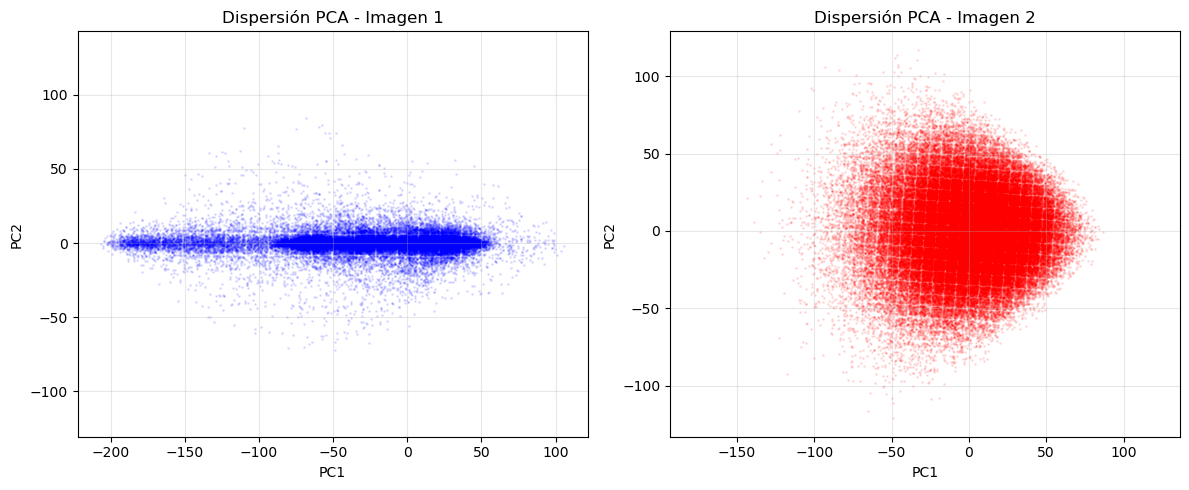
\includegraphics[width=0.8\textwidth]{Ejercicio2.png}
    \caption{Autovalores de los bloques de la imagen y componentes conservados/descartados.}
\end{figure}

\subsection{Descompresión}
\begin{figure}[h!]
    \centering
    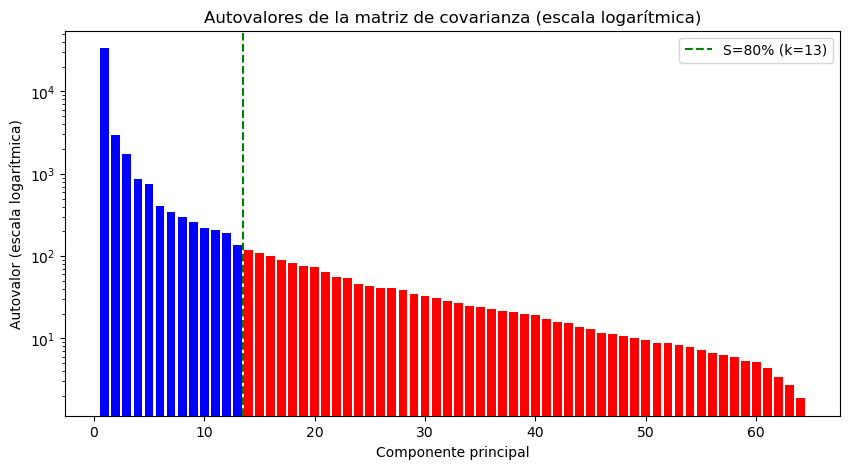
\includegraphics[width=1\textwidth]{Ejercicio3.png}
    \caption{Comparación entre la imagen original y la reconstruida a partir de los vectores comprimidos.}
\end{figure}

\subsection{Medidas de desempeño}
\begin{figure}[h!]
    \centering
    \includegraphics[width=1\textwidth]{Ejercicio4a.png}
    \caption{Error cuadrático medio (MSE) en función del porcentaje de compresión.}
\end{figure}

\begin{figure}[h!]
    \centering
    \includegraphics[width=1\textwidth]{Ejercicio4b.png}
    \caption{Comparación entre distintas imágenes con distintos porcentajes de compresión.}
\end{figure}

% ---------- DISCUSIÓN ----------
\section{Discusión}
Se analizan e interpretan los resultados, comparándolos con expectativas o trabajos previos.

% ---------- CONCLUSIÓN ----------
\section{Conclusión}
Se resumen los hallazgos principales y se sugieren posibles trabajos futuros.

\end{document}
